\textbf{Platforms.} We run our experiments on NERSC Perlmutter~\cite{perlmutter}, 
where each GPU node has four NVIDIA A100 GPUs on a Slingshot-11 interconnect, 
with NVHPC 25.5, CUDA 12.9, cuFFT 11.4, 
and CUDA-aware Cray MPICH 9.1.0. CPU baselines run on the 
Perlmutter's CPU nodes with two 64-core AMD EPYC 7763 (Milan) CPUs each.

\textbf{Cases.} The production case (``wf60'') is a 60-turbine wind
farm of NREL 5-MW reference turbines~\cite{jonkman2009} in a
$10\times6$ array with $7D$ streamwise and $5D$ spanwise spacing
($D=126$\,m), in a $28.2 \times 3.8 \times 2.0$\,km domain discretized
by $3072\times384\times512 \approx 604$M grid points, with the LASD SGS
model, equilibrium wall model, and actuator-line turbines.
Table~\ref{tab:cases} lists the scaling series. Strong scaling runs
the same farm at 512, 768, and 1152 vertical levels (604M, 906M, and
1.36B cells), refining the wall-layer and wake resolution. Weak scaling
fixes the per-GPU grid at three loads and grows the vertical extent with
the GPU count.
We report GPU speedup against the fastest CPU configuration.

\begin{table}[h]
\centering
\caption{Problem sizes of the scaling experiments. Strong scaling keeps
the grid fixed; weak scaling keeps the per-GPU grid fixed.}
\label{tab:cases}
\footnotesize
\setlength{\tabcolsep}{4pt}
\begin{tabular}{@{}lrrl@{}}
\toprule
Grid ($N_x\times N_y\times N_z$) & Cells & Cells/GPU & GPUs \\
\midrule
\multicolumn{4}{@{}l}{\emph{Strong scaling (whole problem)}} \\
$3072\times384\times512$  & 604M  & 37.7M--9.4M  & 16, 32, 64 \\
$3072\times384\times768$  & 906M  & 56.6M--14.2M & 16, 32, 64 \\
$3072\times384\times1152$ & 1.36B & 42.5M--10.6M & 32, 64, 128 \\
\midrule
\multicolumn{4}{@{}l}{\emph{Weak scaling (grid per GPU)}} \\
$3072\times384\times25$ & 118M--1.89B & 29.5M & 4, 8, 16, 32, 64 \\
$512\times512\times40$  & 42M--671M   & 10.5M & 4, 8, 16, 32, 64 \\
$256\times256\times64$  & 16.8M--268M & 4.2M  & 4, 16, 64 \\
\bottomrule
\end{tabular}
\end{table}

\textbf{CPU--GPU backend consistency.}
We first use a small single-turbine case to verify that the CPU and GPU
backends produce consistent LESGO results. Figure~\ref{fig:lesgo-cpu-gpu}
compares matched executions using one NREL 5-MW turbine with a panel-based
actuator-line method and 120 actuator points per blade, with both SGS and
molecular viscosity disabled. Both runs use the same
cold start, $480\times384\times240$ grid, fixed nondimensional time step
$\Delta t=0.0014$, and 1,000 steps. At the common physical time
$t=15.4737$\,s, the transient near-wake fields agree to floating-point
roundoff: the wake-deficit pattern correlation is 1.0, the relative
$L_2$ difference is $1.47\times10^{-13}$, and the maximum normalized axial
velocity difference is $9.00\times10^{-14}$. This test verifies backend
consistency.

\begin{figure*}[t]
\centering
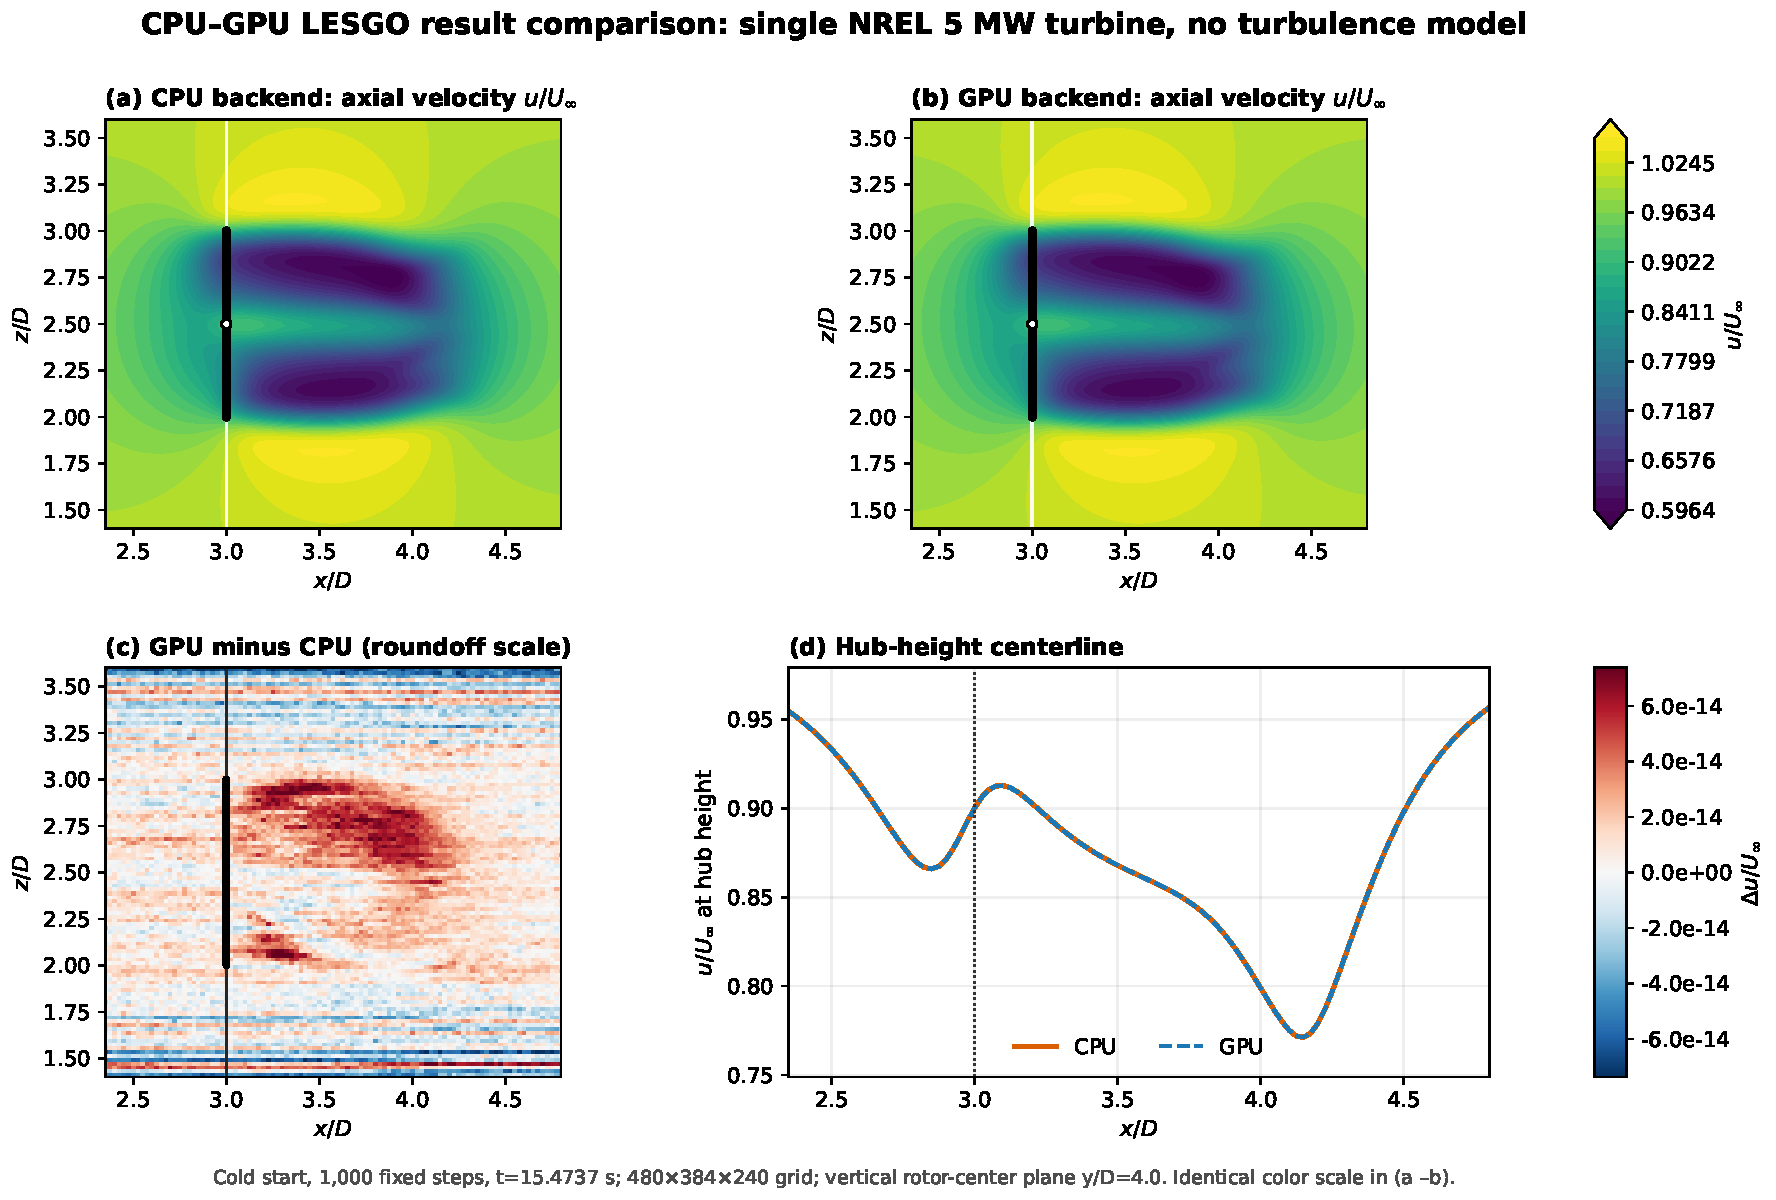
\includegraphics[width=0.96\textwidth]{figs/fig_cpu_gpu_lesgo.pdf}
\caption{Matched CPU--GPU comparison for a 1,000-step LESGO simulation
of one NREL 5-MW turbine at the rated $11.4$\,m\,s$^{-1}$ operating point.
Panels (a) and (b) show normalized axial velocity on the vertical
rotor-center plane using an identical color scale; panel (c) shows the
GPU-minus-CPU difference at roundoff scale; and panel (d) compares the
hub-height centerline profiles. The CPU run used 48 MPI ranks and the GPU run
used two NVIDIA A100 GPUs.}
\label{fig:lesgo-cpu-gpu}
\end{figure*}
